% this template mostly comes from Trinkle23897
% his github repo is https://github.com/Trinkle23897/THU-Beamer-Theme
% thanks a lot Trinkle!
% two color theme fdu_red and fdu_blue
% github repo https://github.com/milanmarks/FDU-Beamer-Theme

\documentclass{beamer}
\usepackage{hyperref}
\usepackage[T1]{fontenc}

% other packages
\usepackage{latexsym,amsmath,xcolor,multicol,booktabs,calligra}
\usepackage{graphicx,pstricks,listings,stackengine}

\author{Zhiyang Liang}
\title{Self Introduction}
\subtitle{}
\institute{School of Data Science, Fudan University}
\date{May 21, 2022}
\usepackage{fdublue}

% defs
\def\cmd#1{\texttt{\color{red}\footnotesize $\backslash$#1}}
\def\env#1{\texttt{\color{blue}\footnotesize #1}}
\definecolor{deepblue}{rgb}{0,0,0.5}
\definecolor{deepred}{rgb}{0.6,0,0}
\definecolor{deepgreen}{rgb}{0,0.5,0}
\definecolor{halfgray}{gray}{0.55}

\lstset{
    basicstyle=\ttfamily\small,
    keywordstyle=\bfseries\color{deepblue},
    emphstyle=\ttfamily\color{deepred},    % Custom highlighting style
    stringstyle=\color{deepgreen},
    numbers=left,
    numberstyle=\small\color{halfgray},
    rulesepcolor=\color{red!20!green!20!blue!20},
    frame=shadowbox,
}


\begin{document}

% \kaishu
\begin{frame}
    \titlepage
    \begin{figure}[htpb]
        \begin{center}
            
\includegraphics[width=0.618\linewidth]{pic/fdu_logo_blue.pdf}
        \end{center}
    \end{figure}
\end{frame}

\begin{frame}
    \tableofcontents[sectionstyle=show,subsectionstyle=show/shaded/hide,subsubsectionstyle=show/shaded/hide]
\end{frame}


\section{Brief Introduction}
    \begin{frame}{Brief Introduction}
        \begin{itemize}
            \item Foundation: Mathematical Analysis, Linear Algebra, Programming, Probability Theory, Mathematical Statistics
            \item Computer Skills: Data Structure, Computer Vision, Neural Network and Deep Learning, Artificial Intelligence
            \item Statistical Skills: Statistical Machine Learning, Regression Analysis, Financial Econometrics, Bayesian Statistics
            \item Honor Course: Advanced Regression Analysis
        \end{itemize}
         
    \end{frame}
    \begin{frame}{Advanced Regression Analysis}
    The name of course may be misleading. It contains many topics of statistics.
        \begin{itemize}
            \item Functional data analysis
            \item High dimensional statistics
            \item Quantile regression
            \item Survival analysis
        \end{itemize}
         
    \end{frame}
\section{High-dim Statistics}

    \begin{frame}{Example of High-dim Data}
    High-frequency financial data have been collected for a host of financial assets, from stocks, bonds, and commodity prices to foreign exchange rates and financial derivatives. \\
    Take China A share market for example:
    \begin{itemize}
        \item Shanghai Stock Exchange (SSE): 1651
        \item Shenzhen Stock Exchange (SZSE): 2259
    \end{itemize}
    The total is 3910.
    \end{frame}

    \begin{frame}{Aim of High-dimensional Statistical Learning}
    The main goals of high dimensional inferences, according to Bickel (2008), are
    \begin{itemize}
        \item construct a method as effective as possible to predict future observations.
        \item gain insight into the relationship between features and responses for scientific purposes, as well as, hopefully, to construct an improved prediction method.
    \end{itemize}
    For selecting stocks, the performance of the procedure is more important than understanding the features. The first goal is more significant.
    \end{frame}
    
    \begin{frame}{Variable Selection}
    Traditionally, we apply:
    \begin{itemize}
        \item a subset selection criterion: Mallows' $C_p$, AIC, BIC...
        \item a subset selection algorithm: best subset selection, forward addition, backward elimination, stepwise regression
    \end{itemize}
    \end{frame}
    
    \begin{frame}{Penalized Least Squares}
    Many of the criteria can be rewritten into penalized form:
    \[
    \frac{1}{2n}\|\mathrm{y}-\mathrm{X}\mathrm{\beta}\|^2+ \lambda\|\mathrm{\beta}\|_0
    \]
    However, the $\|\beta\|_0$ is hard to minimize.
    \end{frame}
    
    \begin{frame}{}
    Breiman (1995) said much work and research have gone into subset selection regression, but the basic method remains flawed by its relative lack of accuracy and instability.\\
    ~\\
    Subset regression either zeros a coefficient, it is is not in the selected subsets, or in flates it. Ridge regression gains its accuracy by selective shrinking. \\
    ~\\
    He argued that methods that select subsets, are stables, and shrink are needed.\\
     ~\\
    That is, a good procedure should be able to select subsets and selectively shrink the coefficients.
    \end{frame}
    
    \begin{frame}{Desired Properties}
        A good penalized LSE should have three properties:
        \begin{itemize}
  	    \item \emph{Sparsity} : The resulting estimator sets small estimate coefficients to zero.
  	    \item \emph{Unbiasedness} : The resulting estimator is nearly unbiased, especially when the true $\beta_j$ is large.
  	    \item \emph{Continuity} : The resulting estimator is continuous in the data to reduce instability in model prediction (Breiman,1996).
        \end{itemize}
    \end{frame}
    
    \begin{frame}{How to achieve the properties}
    	Let $p_\lambda(\theta)$ be nondecreasing and continuously differentiable on $\left [ 0,\infty \right ) $. Assume that the function 
	$-\theta -p'_\lambda(\theta)$ is strictly unimodal on $\left ( 0,\infty \right ) $ with the convention $p'_\lambda(0) = p'_\lambda(0+)$. 
	\begin{itemize}
		\item \emph{Sparsity} : if $\min_{\theta\geq 0 }\{\theta+p'_\lambda(\theta)\} > 0$, which holds if $p'_\lambda(0+) > 0$;
		\item \emph{Approximate Unbiasedness} : if $p'_\lambda(\theta) =0 $ for large $\theta$;
		\item \emph{Continuity} : if and only if $arg\min_{\theta\geq 0}\{\theta+p'_\lambda(\theta)\} = 0$.
	\end{itemize}
    \end{frame}
    
    \begin{frame}{Examples}
     \begin{figure}[H] %H为当前位置,!htb为忽略美学标准,htbp为浮动图形
    \centering %图片居中
    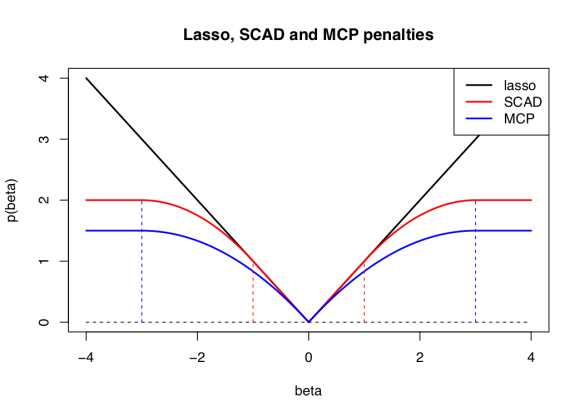
\includegraphics[width=0.7\textwidth]{example.png} %插入图片,[]中设置图片大小,{}中是图片文件名
    \caption{Some examples of nonconcave penalties(compared to lasso)} %最终文档中希望显示的图片标题
    \end{figure} 
    \end{frame}
    
    \begin{frame}{Orthonormal Case}
    \begin{figure}[H] %H为当前位置,!htb为忽略美学标准,htbp为浮动图形
    \centering %图片居中
    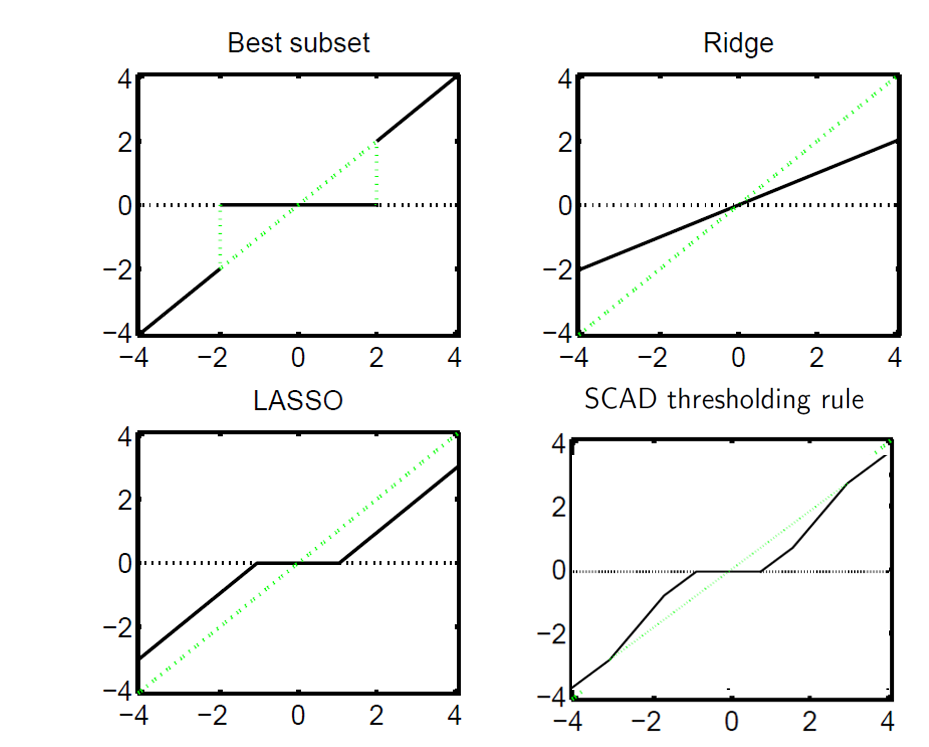
\includegraphics[width=0.7\textwidth]{image.png}
    %插入图片,[]中设置图片大小,{}中是图片文件名
     %最终文档中希望显示的图片标题
    \caption{Results in orthonormal case}
    \end{figure} 
        
    \end{frame}
\section{Summary}
    \begin{frame}{Summary}
    Compared to best subset selection
    \begin{itemize}
        \item faster
        \item more effective
        \item strong theoretical backup
        \item can estimate standard errors of parameters accurately
    \end{itemize}
    Further
    \begin{itemize}
        \item LASSO has good performance when noise to signal ratio is large, but bias is large
        \item SCAD gives the best performance in selecting significant variables without excessive bias
        \item Approach can be applied to other statistical contexts
    \end{itemize}
    
    \end{frame}
    \begin{frame}{Summary}
    \begin{center}
        {\Huge\calligra Thanks!}
    \end{center}
    \end{frame}


\end{document}